\documentclass[10pt]{article}
\usepackage{fullpage,enumitem,amsmath,amssymb,graphicx}
\usepackage{tikz}
\usepackage{array}
\usepackage{verbatim}

\begin{document}

\begin{center}
{\Large CS224N Winter 2016 Homework [3]}

\begin{tabular}{rl}
SUNet ID: & [jiajuns, xxx, xxx] \\
Name: & [Jiajun Sun, Sijun He, Mingxiang Chen] \\
\end{tabular}
\end{center}

By turning in this assignment, I agree by the Stanford honor code and declare
that all of this is my own work.

\section*{Problem 1: A window into NER}
\begin{enumerate}[label=(\alph*)]
\item
i.\\
Yesterday, price of Apple increased 6.56 percent.\\
Here apply can be interpreted as Apple the company or apple the fruit.\\
\\
Calvin Klein just released some nice designs for the winter season.\\
Here Calvin Klein can be interpreted as a name or a company.\\
\\

ii.\\
Words alone can have ambiguity, therefore adding features other than the word itself can help reduce ambiguity.\\
\\

iii.\\
First, the context of the word can help. The words around can imply the correct meaning of the center word.
Second, dependence structure within the window could shed light on the function of the center word in the sentences, which helps interpreting its entity.

\item
i.\\
$e^{(t)}$ has dimension of $1 \times 2(w+1)D$\\
$W$ has dimension of $2(w+1)D \times H$\\
$U$ has dimension of $H \times C$\\
\\
ii.\\
$$
\begin{aligned}
& cost(ReLu) = \mathcal{O}(H) + \mathcal{O}(2(w+1)D \times H)\\
& cost(softmax) = \mathcal{O}(H \times C) + \mathcal{O}(C)\\
& cost(CE) = \mathcal{O}(C)
\end{aligned}
$$
Given the sentences has length of $T$, the computation complexity is:
$$
\begin{aligned}
cost
& = T \times \mathcal{O}(\mathcal{O}(H) + \mathcal{O}(2(w+1)D \times H) + \mathcal{O}(H \times C) + \mathcal{O}(C) + \mathcal{O}(C))\\
& \approx \mathcal{O}(2(w+1)D \times H \times T)\\
& \approx \mathcal{O}(wDHT)
\end{aligned}
$$

\item
(code)

\item
i.\\
Entity level P/R/F1: 0.82/0.84/0.83\\
The confusion matrix shows that the model has a very low false positive rate of misclassifying null class into an entity. Among all the entities,  ORG has the lowest accuracy.
\begin{table}[h]
	\centering
	\caption{confusion matrix}
	\begin{tabular}{|l|l|l|l|l|l|}
	\hline
	Acutal \textbackslash Predicted & PER     & ORG     & LOC     & MISC    & O        \\ \hline
	PER   & 2940.00 & 56.00   & 46.00   & 13.00   & 94.00    \\ \hline
	ORG   & 128.00  & 1676.00 & 92.00   & 63.00   & 133.00   \\ \hline
	LOC   & 54.00   & 119.00  & 1845.00 & 29.00   & 47.00    \\ \hline
	MISC  & 36.00   & 63.00   & 35.00   & 1018.00 & 116.00   \\ \hline
	O     & 37.00   & 42.00   & 12.00   & 31.00   & 42637.00 \\ \hline
	\end{tabular}
\end{table}

ii.\\
The first limitation is that the length of context is limited by the length of window size.
For example the \textbf{Test and County Cricket Board} does not get right label, because the length has exceeded the window size.\\
\\
The second limitation is that the model is too simplistic. The context is based solely on concatenating word vectors. The model can't decide which word in the context should it focus on. For example, \textbf{Grace Road} was not correctly classified in ``at Grace Road". The word ``at" is a very strong signal that the next word/phrases should be locations but the model fails to capture that. Currently the word ``at" has the same effect anywhere within the window. With a more sophisticated model like LSTM or GRU, we should be able to put emphasis on words that are more relevant to the entity. 

\end{enumerate}
\clearpage
\section*{Problem 2:RNN for NER}
\begin{enumerate}[label=(\alph*)]
\item
i.\\
The number of RNN parameters:
$$
V \times D + H \times H + D \times H + H + H \times C + C
$$
The number of window-based model parameters:
$$
V \times D + D \times H + H + H \times C + C
$$
Therefore, RNN has $HH$ more parameters than window-based model.\\

ii.\\
Cost for one time step:
$$
\begin{aligned}
& cost(h) = \mathcal{O}(H \times H) + \mathcal{O}(D \times H) + \mathcal{O}(H)\\
& cost(softmax) = \mathcal{O}(H \times C) + \mathcal{O}(C)\\
& cost(CE) = \mathcal{O}(C)
\end{aligned}
$$
Adding them up:
$$
\mathcal{O}(H \times H) + \mathcal{O}(D \times H) + \mathcal{O}(H) + \mathcal{O}(H \times C) + \mathcal{O}(C) + \mathcal{O}(C) \approx \mathcal{O}(H \times H) + \mathcal{O}(D \times H)
$$
Therefore the total cost for sentence of length $T$:
$$
cost = T(\mathcal{O}(H \times H) + \mathcal{O}(D \times H))
$$

\item
i.\\
Consider a dataset that most of (over $90\%$) the entity is person,
if the model label all the entity as person the cross entropy error should be smaller.
However, by doing this the $F_1$ score should drop, because the prediction is biased and recall value will drop.

ii.\\
Optimizing $F_1$ score requires looking through the entire training set. The cost and memory requirement is huge.

\item
(code)

\item
The padded label $y$ will be transform into a one-hot vector.
When $y=0$, the corresponding one-hot vector is $[1, 0, 0, 0, 0]$.
Therefore, the padded label will be considered as label $o$.
The cross entropy loss is not always zero for the padded part.

\item
(code)

\item
result:

\item
explanation:

\end{enumerate}
\clearpage
\section*{Problem 3:Grooving with GRUs}
\begin{enumerate}[label=(\alph*)]
\item
i.\\
$U_h = 1$, $W_h = 1$ and $b_h = 0$ will allow the RNN to replicate this behavior.\\

ii.\\
$U_z = 0$, $W_z = 1$, $U_h = 1$ and $W_h$ can be any value.\\
When $x=0$, $z_t = 0$ and $\tilde{h_t} = 0$ thus the hidden state will always be $h_t = 0$.
Whenever $x=1$, $z_t = 0$ and the hidden state will keep to be $h_t = h_{t-1} = 1$.

\item
i.\\
It is impossible for RNN to have togging behavior.
$U_t$ has to be a positive number in order to let $h_t$ switch to $1$.
Therefore for the second time when $x = 1$ it is impossible to let $h_t$ switch back to $0$.\\

ii.\\
$b_r = 1$, $U_z = -1$, $W_z = 1$, $U_h = 1$ and $W_h = -1$.
When $x=0$, $z_t = 0$ and $\tilde{h_t} = 0$ thus the hidden state will always be $h_t = 0$.
When $x=1$ for the first time, $z_t = 0$ but $\tilde{h_t} = 1$ thus the hidden state will switch to $h_t = 1$.
If $h_t=1$ and $x=0$, $z_t = 1$ and hidden state $h_t = h_{t-1} = 1$.
But if $x=1$, $z_t = 0$ and hidden state $h_t = \tilde{h_t} = 0$.

\item
(code)

\item
\begin{figure}[h]
\center
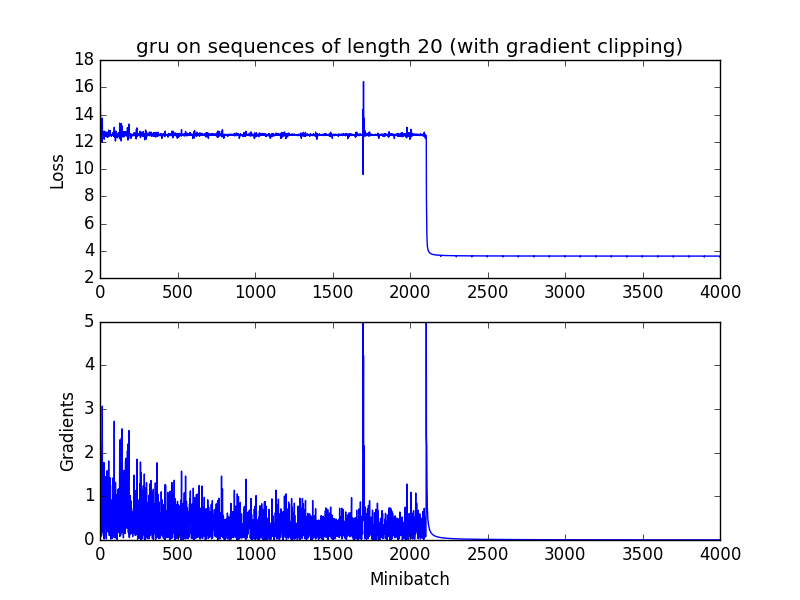
\includegraphics[scale=0.45]{q3-clip-gru.png}
\end{figure}

\begin{figure}[h]
\center
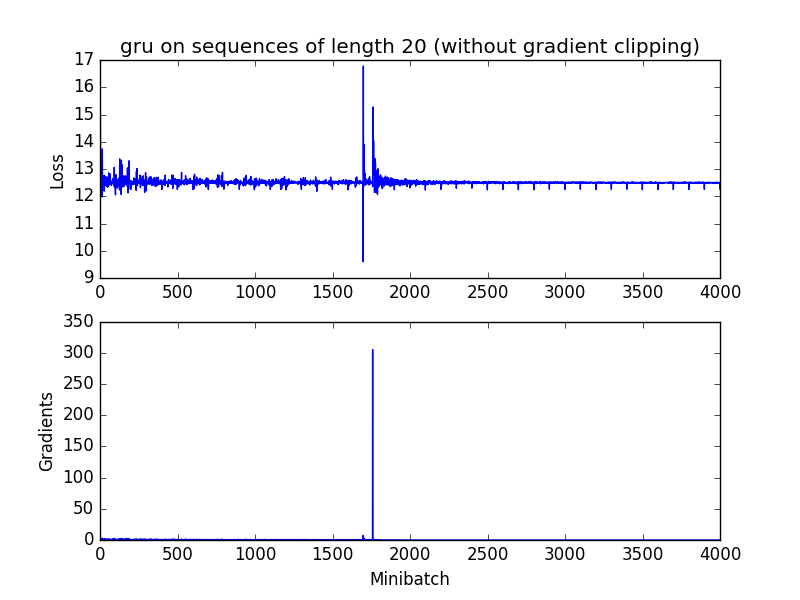
\includegraphics[scale=0.45]{q3-noclip-gru.png}
\end{figure}

\begin{figure}[h]
\center
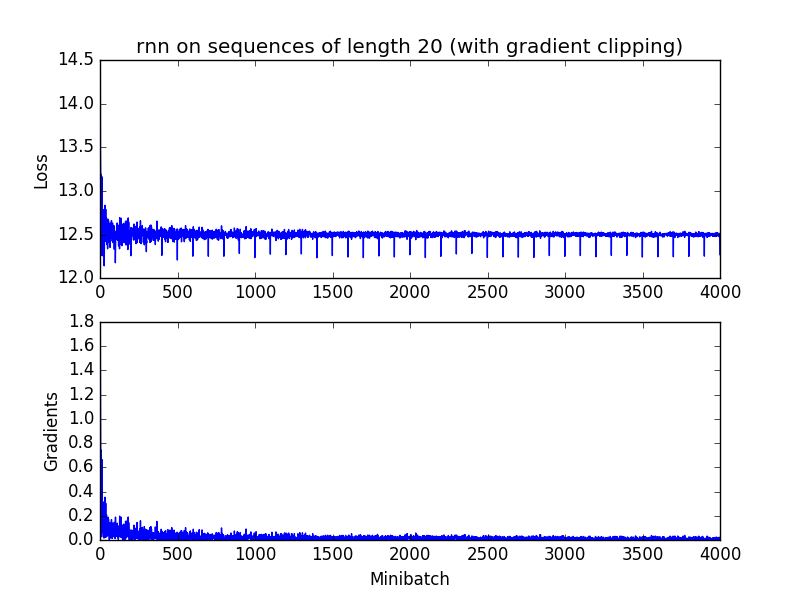
\includegraphics[scale=0.45]{q3-clip-rnn.png}
\end{figure}

\begin{figure}[h]
\center
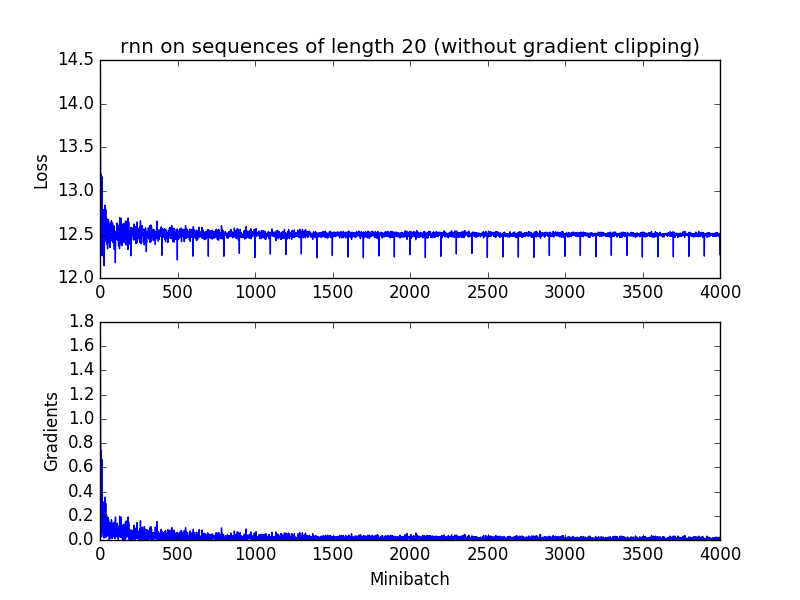
\includegraphics[scale=0.45]{q3-noclip-rnn.png}
\end{figure}

\item
explanation:

\item
waiting for the GPU then we can train this
F1 score


\end{enumerate}


\end{document}

